%% LyX 2.3.7 created this file.  For more info, see http://www.lyx.org/.
%% Do not edit unless you really know what you are doing.
\documentclass[english,notitlepage]{revtex4-1}
\usepackage[T1]{fontenc}
\usepackage[latin9]{inputenc}
\setcounter{secnumdepth}{3}
\usepackage{amsmath}
\usepackage{amssymb}
\usepackage{babel,graphicx,listings,color}
\begin{document}
\title{Analysing sound wave using fast Fourier transform}
\maketitle

\section{Sound wave}

A sound wave consists of compression and rarefaction of air molecules, which travels through space with sound speed $c_s$.
Fig.~\ref{fig:sound-wave} depicts the propagation of a \emph{sinusoidal} sound wave inside an infinitely long rectangular channel.
The figure shows the snapshots of the air molecules (represented by the blue dots in the figure) at four different instantaneous time $t=0\,\text{s}$, $0.001\,\text{s}$, $0.002\,\text{s}$, and $0.003\,\text{s}$.
The regions of high density are called the compression regions (these look like fuzzy vertical blue bands in the figure) and the regions of low density are called the rarefaction regions.
In the figure, these bands of compression and rarefaction regions travel along the positive $x$-direction with speed equals to the sound speed $c_s$.
The wavelength of this sinusoidal sound wave is defined by the distance between two nearest compression bands, which is equal to $\lambda=2\,\text{m}$.
As we can see from the figure, after time $t=0.003\,\text{s}$, the bands will have travelled a distance of $1\,\text{m}$.
Therefore the speed of sound in this example is equal to:
\begin{equation}
c_s = \frac{1\,\text{m}}{0.003\,\text{s}} \simeq 333\,\text{ms}^{-1}.
\end{equation}
In general, the speed of sound depends on various factors such as ambient pressure and temperature.

\begin{figure}[h]
\centering
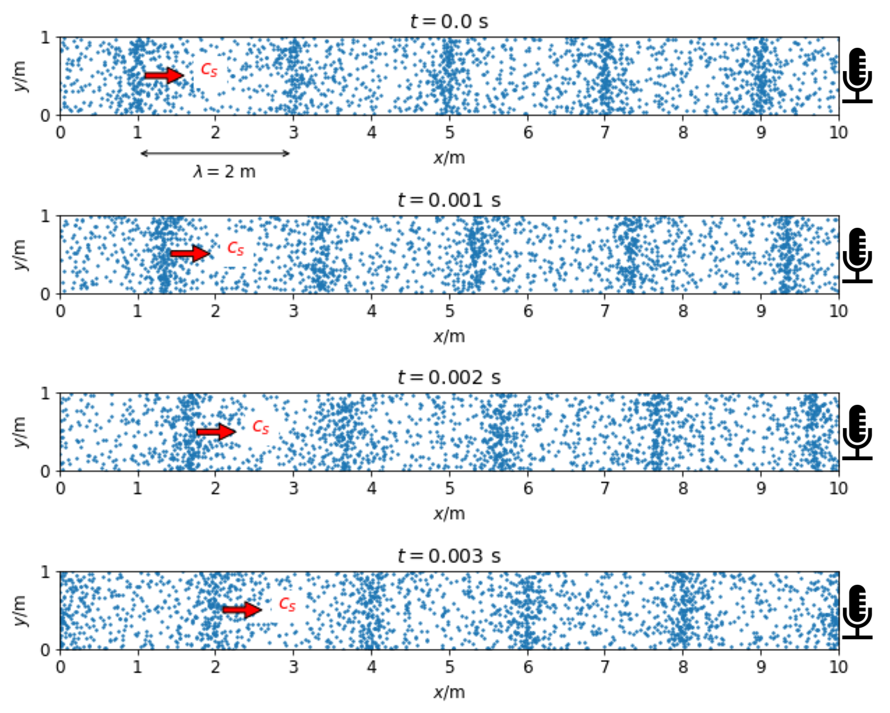
\includegraphics[width=0.7\columnwidth]{./figures/sound-wave.pdf}
\caption{A sinusoidal sound wave travelling to the right with sound speed $c_s$ and wavelength $\lambda$.
Top to bottom indicate the snapshots of the air molecules at four instantaneous times.}
\label{fig:sound-wave}
\end{figure}

Now suppose that that we place a microphone at the end of the channel.
The compression and rarefaction of air will cause the diaphragm inside the microphone to vibrate.
This vibration is then converted into an electrical signal, which is shown in Fig.~\ref{fig:sinusoidal}.
The horizontal axis in the figure represents the time $t$ (in units of seconds).
The vertical axis represents the voltage of the electrical signal produced by the microphone $V(t)$ (in some rescaled units, which we do not need to worry about).
As we can see in this example, the audio signal in Fig.~\ref{fig:sinusoidal} has a sinusoidal form, which can be described by a trigonometric function:
\begin{equation}
V(t) = A\cos(\omega t + \phi),
\end{equation}
where $V(t)$ is the audio signal (in some rescaled units), $t$ is time (in seconds), $A$ is the amplitude, $\omega$ is the angular frequency, and $\phi$ is the phase difference.
The angular frequency $\omega$ is related to the frequency $f$ and period $T$ of the sound wave through this relation:
\begin{equation}
\omega = 2\pi f = \frac{2\pi}{T}. 
\end{equation}
From the plot below, we can measure the period to be $T=0.006\,\text{s}$, which translates to audio frequency of $f=\frac{1}{T}\simeq167\,\text{Hz}$.
Hz (pronounced as Hertz) is the SI unit of frequency, defined to be $\text{Hz}=\text{s}^{-1}$.

In the equation above, $V$, $A$, $\omega$, $\phi$, and $t$ are all real. 
However, sometimes it might be useful to write the audio signal in a complex form (as we shall see later in Fourier series) as follows:
\begin{equation}
V(t) = C e^{i\omega t} + C^{*} e^{-i\omega t} \text{, where $C=\frac{A}{2}e^{i\phi}$ is the complex amplitude (the rest of the variables are real).}
\end{equation}
The star $*$ above $C$ indicates complex conjugate operation.

\begin{figure}[h]
\centering
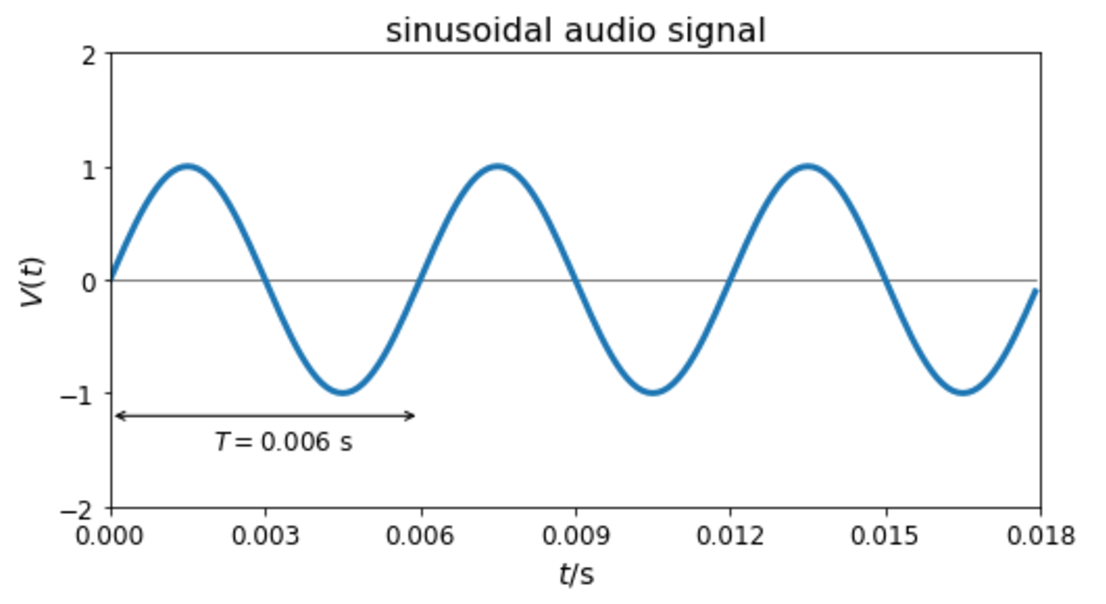
\includegraphics[width=0.6\columnwidth]{./figures/sinusoidal.pdf}
\caption{A sinusoidal audio signal with period $T=0.006\,\text{s}$ and frequency $f=\frac{1}{0.006\,\text{s}}\simeq167\,\text{Hz}$.}
\label{fig:sinusoidal}
\end{figure}

\section{Fourier series}

In Fig.~\ref{fig:sinusoidal}, the audio signal can be described by a single trigonometric function.
This is because we have assumed the sound wave to be sinusoidal.
However this is not true in general.
For example, the sound wave coming from a tuning fork is very close to a sinusoidal wave,
on the other hand, the sound wave from a saxophone is far from being sinusoidal.

Let us consider another audio signal from an unknown musical instrument, which is depicted in Fig.~\ref{fig:Fourier-series} top.
We can immediately tell that the signal is periodic with the same period $T=0.006\,\text{s}$ (or fundamental frequency $f\simeq167\,\text{Hz}$) as the one in Fig.~\ref{fig:sinusoidal}.
However, the shape of the audio signal in Fig.~\ref{fig:Fourier-series} is much more complicated than a sinusoidal wave and cannot be simply described by a single trigonometric function.
Luckily, Fourier series allows us to decompose this periodic signal into a sum of trigonometric functions as follows:
\begin{equation}
V(t) = \sum_{p=-\infty}^{\infty} C_p e^{i\omega_p t} \text{, where }\omega_p=\frac{2\pi p}{T} \text{ and } p\in\mathbb{Z}.
\end{equation}
Each term in the Fourier series is a simple sinusoidal wave with angular frequency $\omega_p$ and
complex amplitude $C_p$'s.
The first non-constant term in the Fourier series corresponds to the \emph{fundamental frequency}
$\omega_1 = \frac{2\pi}{T}$ shown by first plot in the second row of Fig.~\ref{fig:Fourier-series}.
The next term in the Fourier series has double the fundamental frequency $\omega_2=\frac{4\pi}{T}$ 
and is sometimes called the second harmonic (see second plot in the second row of Fig.~\ref{fig:Fourier-series}). 
The next next term has triple the fundamental frequency $\omega_3=\frac{6\pi}{T}$ and is sometimes called the third harmonic (see third plot in the second row of Fig.~\ref{fig:Fourier-series}).

To find the complex amplitudes $C_p$'s (or Fourier coefficients) we multiply the above equation by $e^{-i\omega_q t}$ and then integrate with respect to $t$ from $t=0$ to $t=T$.
\begin{equation}
\int_0^T V(t) e^{-i\omega_q t}\,dt = \sum_{p=-\infty}^{\infty} C_p \int_0^T e^{i(\omega_p - \omega_q) t}\,dt,
\end{equation}
where $p$ and $q$ are integers.
We note that the integral:
\begin{equation}
\int_0^T e^{i(\omega_p - \omega_q) t}\,dt = \int_0^T e^{i\frac{2\pi}{T}(p-q) t}\,dt =
\begin{cases}
T & \text{if } p = q \\
0 & \text{if } p \neq q
\end{cases}.
\end{equation}
More succintly, we can write,
\begin{equation}
\int_0^T e^{i(\omega_p - \omega_q) t}\,dt = T \delta_{pq},
\end{equation}
where the Kronecker delta $\delta_{pq}$ is defined to be equal to $1$ if $p=q$ and $0$ if $p\neq q$.
Therefore,
\begin{align}
\int_0^T V(t) e^{-i\omega_q t}\,dt &= \sum_{p=-\infty}^{\infty} C_p T \delta_{pq} = T C_q \\
\Rightarrow C_q &= \frac{1}{T} \int_0^T V(t) e^{-i\omega_q t}\,dt.
\end{align}

\textbf{Question 1.}
(a) Show that if $C_{-p}=C_p^*$ for all $p\in\mathbb{Z}$, then $V(t)$ is real.
(b) Show that if $V(t)$ is real, then $C_{-p}=C_p^*$ for all $p\in\mathbb{Z}$.

\begin{figure}[h]
\centering
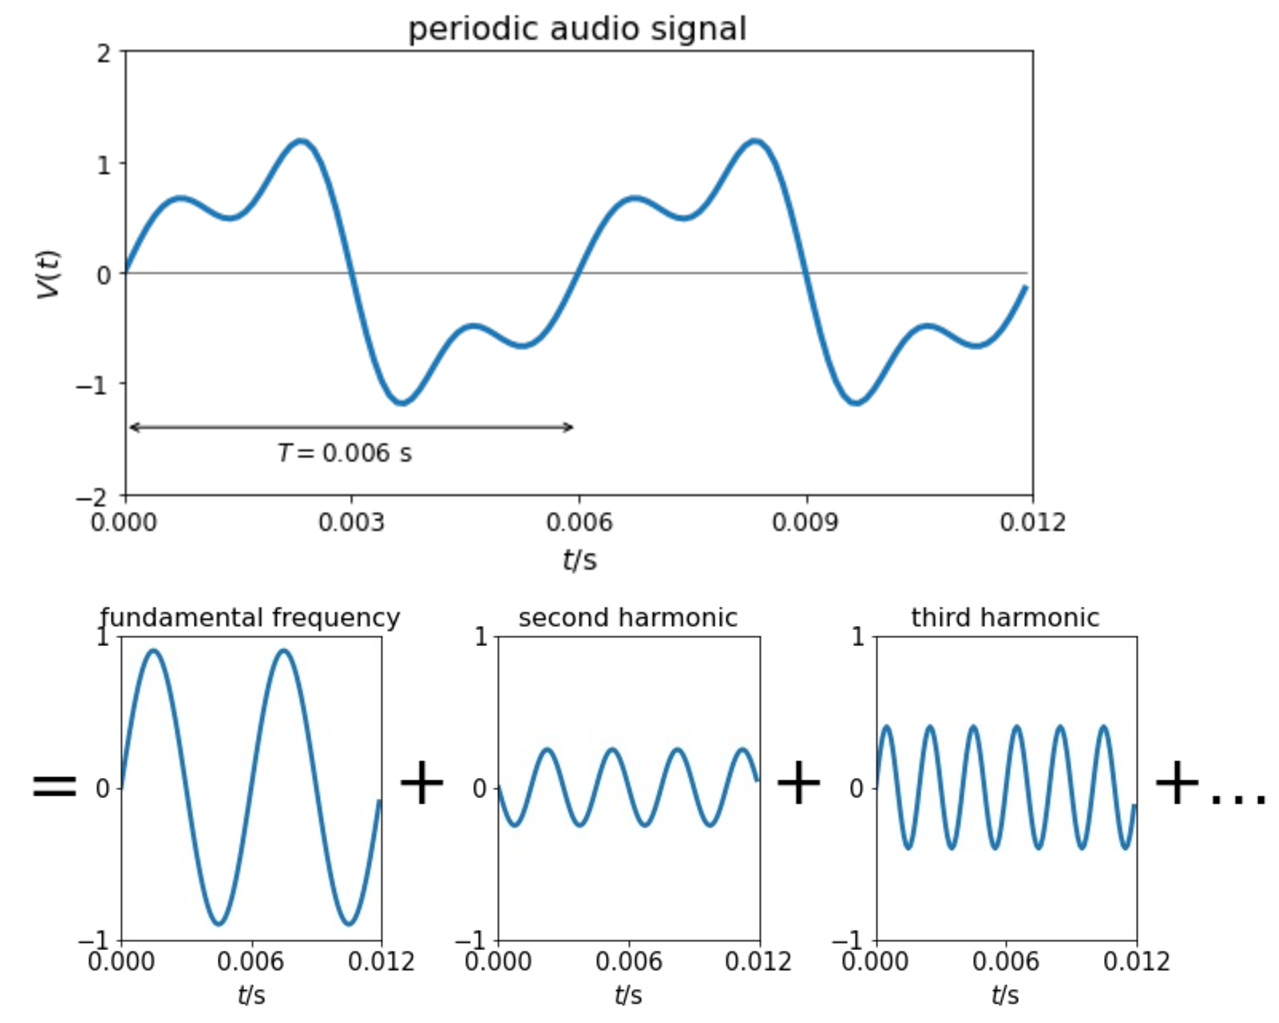
\includegraphics[width=0.7\columnwidth]{./figures/Fourier-series.pdf}
\caption{Any periodic function can be decomposed into an infinite sum of trigonometric function with frequency doubling in each subsequent term (Fourier series). 
The first term in the Fourier series has the frequency equals to the original function (fundamental frequency).}
\label{fig:Fourier-series}
\end{figure}

\section{Fourier transform}

In reality, the audio signal is not perfectly periodic since it might be contaminated by a background noise. 
Furthermore the oscillation of the sound wave itself decays gradually to zero, 
so a realistic representation of an audio signal recorded from a microphone might look something like Fig.~\ref{fig:Fourier-transform}(a).

To analyse this audio signal, we shall use Fourier transform, which is an extension of the Fourier series above by taking the limit $T\rightarrow\infty$ (loosely speaking, the function $V(t)$ is no longer periodic).
In this case the angular frequency of each Fourier component becomes continuous $\omega_p\rightarrow\omega\in\mathbb{R}$.
The Fourier transform of $V(t)$ is another function $\tilde{V}(\omega)$, which is a function of angular frequency $\omega$.
$V(t)$ and $\tilde{V}(\omega)$  are related through the following relations:
\begin{align}
V(t) &= \int_{-\infty}^\infty \tilde{V}(\omega) e^{i\omega t} d\omega 
\quad\text{(inverse Fourier transform)}\\
\tilde{V}(\omega) &= \frac{1}{2\pi}\int_{-\infty}^\infty V(t) e^{-i\omega t} dt
\quad\text{(Fourier transform),}
\end{align}
where $\omega\in\mathbb{R}$.
The above relations can be derived by taking the limit $T\rightarrow\infty$ in the definition of Fourier series, in which case the summation over $\omega_p$ becomes an integral over $\omega$, and then relabelling $C_p \rightarrow \tilde{V}(\omega_p) \rightarrow \tilde{V}(\omega)$.

Now let us define the Dirac delta function $\delta(x - y)$, where $x,y\in\mathbb{R}$ such that
\begin{equation}
\delta(x - y) = 
\begin{cases}
0 &\text{if } x\neq y \\
\infty &\text{if } x = y
\end{cases}.
\end{equation}
The Dirac delta function has the following properties:
\begin{equation}
\int_{-\infty}^\infty \delta(x - y)\,dx = 1, \quad\text{and}\quad 
\int_{-\infty}^\infty \delta(x - y)f(x)\,dx = f(y).
\end{equation}
In continous space, though it is ill-defined, its graph would take the shape of an infinitely thin curve that peaks at a single point, $x = y$, and is zero elsewhere. 
The area (integral) under this curve is equal to $1$, see the second figure below.


\textbf{Question 2.}
Using the definition of Fourier transform, show that
\begin{equation}
\int_{-\infty}^\infty e^{i (\alpha - \beta) t} \,dt = 2\pi \delta(\alpha - \beta),
\end{equation}
for all $\alpha,\beta,t\in\mathbb{R}$.

\textbf{Question 3.}
Show that if $V(t)$ is real then $\tilde{V}(-\omega)=\tilde{V}(\omega)^*$ for all $\omega\in\mathbb{R}$ and \emph{vice versa}.

\begin{figure}[h]
\centering
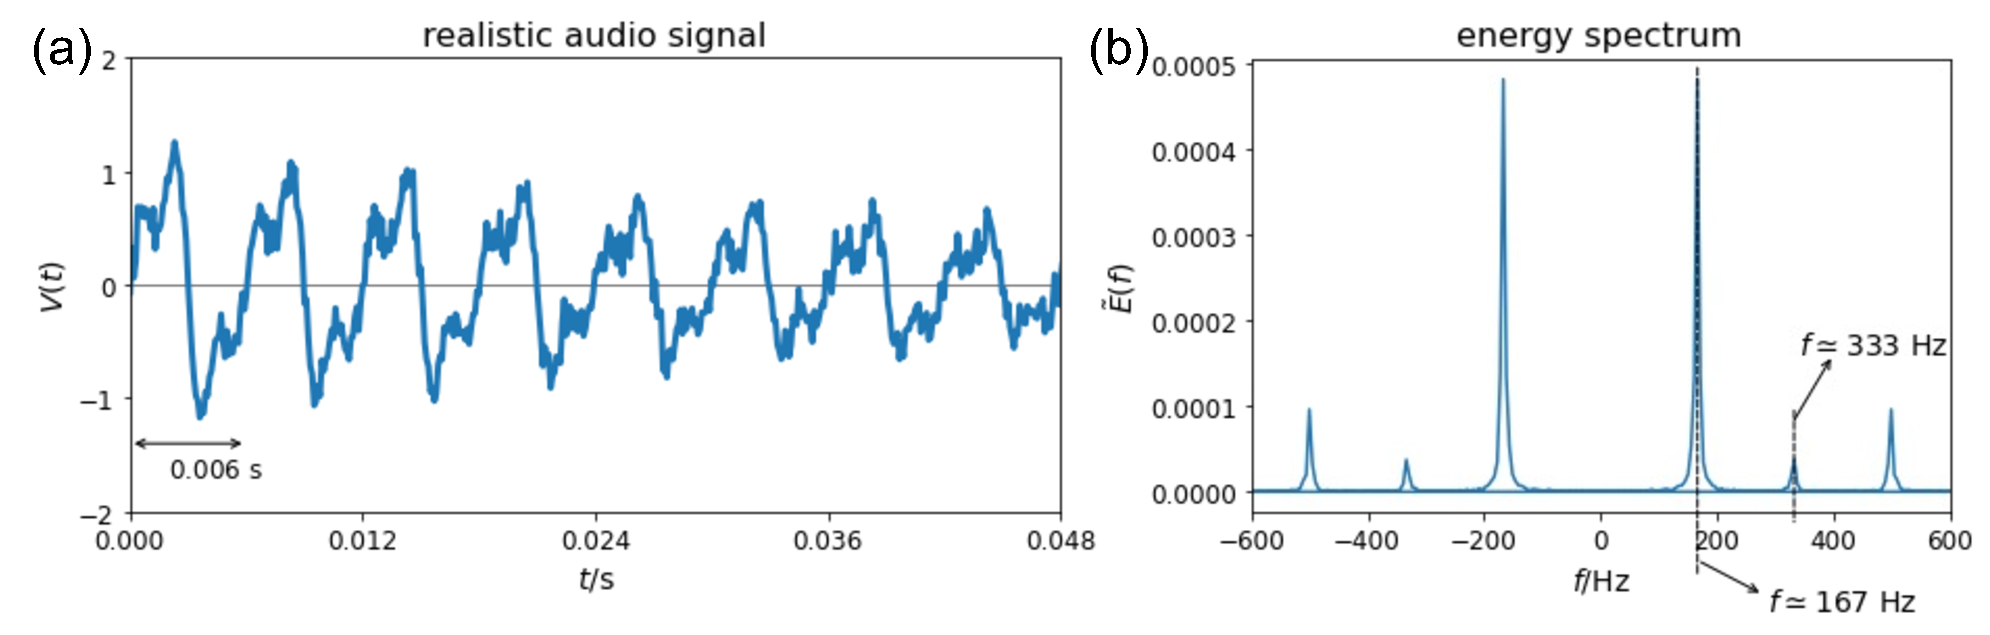
\includegraphics[width=1.0\columnwidth]{./figures/Fourier-transform.pdf}
\caption{(a) shows a typical noisy audio signal. (b) shows the corresponding energy spectrum. The energy spectrum shows several sharp peaks. The first peak corresponds to the fundamental frequency $f=\frac{1}{0.006\,\text{s}}\simeq167\,\text{Hz}$.}
\label{fig:Fourier-transform}
\end{figure}

\section{Energy spectrum}

From electromagnetism, we learnt that the rate of power dissipation is given by:
\begin{equation}
P(t) = \frac{V(t)^2}{R},\quad\text{where $R$ is the electrical resistance.}
\end{equation}
The total energy dissipation is then given by the integral
\begin{equation}
E = \frac{1}{R}\int_{-\infty}^\infty V(t)^2\,dt
\end{equation}
Substituting the definition for Fourier transform to the above, we get:
\begin{align}
E &= \frac{1}{R} \int dt \int d\omega \int d\omega' \, \tilde{V}(\omega)\tilde{V}(\omega') e^{i (\omega + \omega') t} \\
&= \frac{2\pi}{R} \int d\omega \int d\omega' \, \tilde{V}(\omega)\tilde{V}(\omega') \delta(\omega + \omega') \\
&= \frac{2\pi}{R} \int d\omega \, \tilde{V}(\omega) \tilde{V}(-\omega) 
\end{align}
Since $V(t)$ is real, we have $\tilde{V}(-\omega)=\tilde{V}(\omega)^*$ from the previous exercise
and thus the total energy dissipation can be written as:
\begin{equation}
E = \frac{2\pi}{R} \int_{-\infty}^\infty d\omega \, |\tilde{V}(\omega)|^2 
\end{equation}
Now we can define the energy spectrum to be $\tilde{E}(\omega)=|\tilde{V}(\omega)|^2$.
Physically, Fourier transform allows us to decompose an electrical signal into an infinite sum of sinusoidal oscillations with different angular frequencies $\omega$'s.
The energy spectrum $\tilde{E}(\omega)$ gives the energy contribution from a single oscillation with particular angular frequency $\omega$.

Fig.~\ref{fig:Fourier-transform}(b) shows the energy spectrum $\tilde{E}(f)$ as a function of frequency $f$, which corresponds to the noisy audio signal $V(t)$ in Fig.~\ref{fig:Fourier-transform}(a).
Note that the frequency $f$ is related to the angular frequency by a factor of $2\pi$, \emph{i.e.} $\omega=2\pi f$.
As we can see in the figure below, the energy spectrum spectrum is symmetric with respect to $f\rightarrow-f$
(and for this reason, $\tilde{E}(f)$ is usually plotted on the positive $x$-axis only).
Furthermore we also observe several sharp peaks in the energy spectrum.
The first peak $f\simeq167\,\text{Hz}$ corresponds to the fundamental frequency of the signal.
(Although the signal is no longer periodic, it still retains some underlying periodic characteristics.)
The second peak $f\simeq333\,\text{Hz}$ (which is double the fundamental frequency) corresponds to the second harmonic and so on.

\textbf{Question 4.}
Show that the energy spectrum is symmetric, \emph{i.e.} $\tilde{E}(\omega)=\tilde{E}(-\omega)$. 

\section{Discrete Fourier transform}

TO BE ADDED LATER

\begin{figure}[h]
\centering
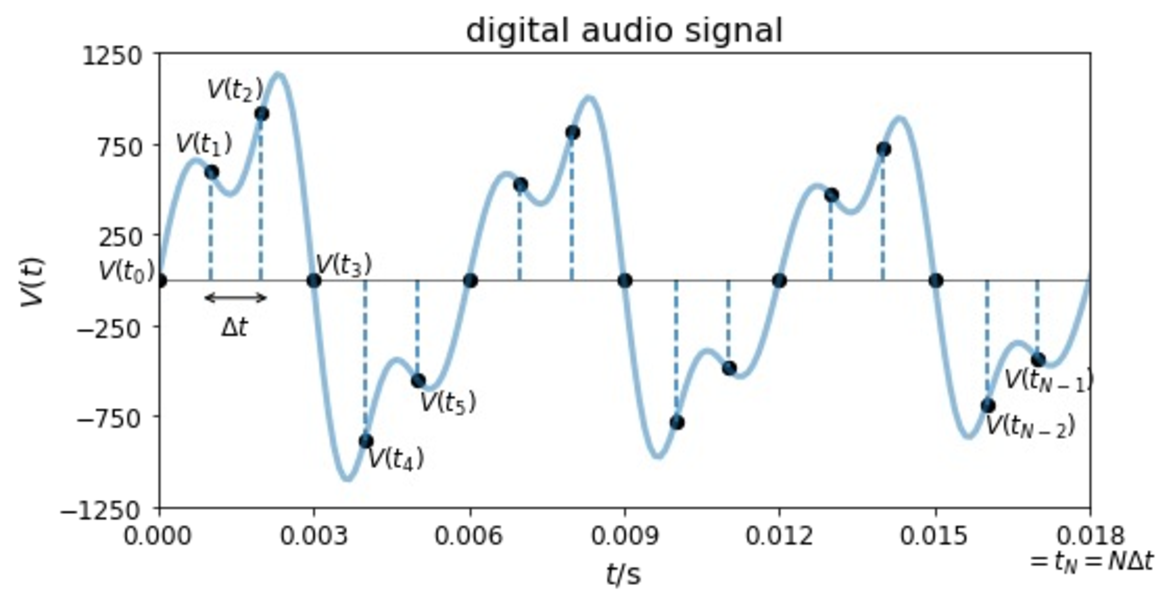
\includegraphics[width=0.7\columnwidth]{./figures/digital-audio.pdf}
\caption{In computer, the audio signal $V(t)$ is discretized into a finite set of points $\{V(t_0),V(t_1),\dots V(t_{N-1})\}$.}
\label{fig:digital-audio}
\end{figure}

\section{Storing audio wave into a computer}

Let's say we record a sound on our microphone for the total duration of $t_N$ (also called the sampling time). 
How is this audio signal $V(t)$ stored inside our computer?
Obviously a computer cannot store an infinite amount of information, so the computer has to divide the signal $V(t)$ into discrete values $V(t_0),V(t_1),V(t_2),\dots,V(t_{N-1})$ at discrete times $t_n$'s, as we can see in Fig.~\ref{fig:digital-audio}.
This also means that the time is discretized into:
$t\rightarrow t_n=n\Delta t$, where $n=0,1,2,\dots,N-1$ and $\Delta t$ is the timestep.
In Fig.~\ref{fig:digital-audio}, the total time (or sampling time) is $t_N=0.018\,\text{s}$, the timestep is $\Delta t = 0.001\,\text{s}$, and the total number of points is $N=18$.
We also define the framerate to be the total number of points $N$ per unit time.
In Fig.~\ref{fig:digital-audio}, we can calculate the framerate to be:
\begin{equation}
\text{framerate} = \frac{N}{t_N} = \frac{18}{0.018\,\text{s}} = 1000\,\text{s}^{-1}.
\end{equation}
Usually, when we record a sound using recording software such as Audacity, we need to specify this framerate.
Higher framerate will give a better sound quality but the file size will also be bigger!
For a 16-bit digital audio, the values of $V$ ranges from $-32768$ to $32767$ in integer steps (note that $V(t)$ is in some rescaled units).
Therefore the vertical $V$-axis in Fig.~\ref{fig:digital-audio} is also discrete. 

\section{Importing .wav file}

There are different audio formats in computer such as {\color{blue} .mp3} and {\color{blue} .wav}.
The difference is that the former is a compressed file while the later is an uncompressed file.
In this Tutorial, we will only consider `.wav` files. 

Let us now put everything we have learnt above into practice. 
Inside the folder {\color{blue} "./samples/"} we have various {\color{blue} .wav} files from different notes from different musical instruments.
First let us have a look at the file called {\color{blue} "./samples/piano-C4.wav"}. 
This is a recording of the note C4 in a piano.
This note has a fundamental frequency of $261.63\,\text{Hz}$.
Let us now analyse this wave file below.
First we need to import the essential libraries such as {\color{blue} numpy}, {\color{blue} matplotlib}, {\color{blue} sys} and {\color{blue} wave} into Python, 
as you can see in the first few lines of the code below.
The library {\color{blue} sys} is used to access the filesystem inside our computer and the library {\color{blue} wave} is used to import and export {\color{blue} .wav} files.
Next we will open the file {\color{blue} "./samples/piano-C4.wav"} and store it into an object, called {\color{blue} inputfile},
using the method {\color{blue} wave.open("./samples/piano-C4.wav", "r")}.
The letter {\color{blue} "r"} indicates that we are reading the file (while the letter {\color{blue} "w"} indicates writing into a file). 
Before we proceed further, we need some information about this audio signal, which we just imported.
For example, we need the framerate, which we can obtain using the method {\color{blue} .getframerate()}. 
In this case the framerate is $11025\,\text{s}^{-1}$, which we can confirm by printing the value into the screen.
We also need the total number of points, \emph{i.e.} $N$, which we can obtain using the method {\color{blue} .getnframes()}.
In this case we get $N=29750$.
Hence we can calculate the total recording time (or sampling time) $t_N$:
\begin{equation}
t_N = \frac{N}{\text{framerate}} \simeq 2.70\,\text{s}.
\end{equation}
We also need to compute the timestep $\Delta t$:
\begin{equation}
\Delta t = \frac{t_N}{N} = \frac{1}{\text{framerate}} \simeq 0.0000907\,\text{s}.
\end{equation}

To read the actual audio signal itself from the {\color{blue} .wav} file, we use the method {\color{blue} .readframes(-1)}.
If you try to print the output you will get something like this:
{\color{blue} b'\textbackslash xf6\textbackslash xf1\textbackslash xff\textbackslash xf1\textbackslash xff...\textbackslash xf2\textbackslash xff'}.
The strange combination of three characters, separated by backslash, actually represents a binary number.
We need to convert these binary numbers, called bytes objects, into decimals using the numpy method {\color{blue} np.frombuffer(V, dtype=np.int16)}.
The {\color{blue} int16} data type indicates that it is a 16-bit audio, so that the values of $V$ ranges from $-32768$ to $32767$ in integer steps.

To plot the the audio signal $V(t)$ as a function of time $t$ we use the library {\color{blue} matplotlib.pyplot}.
First we need to define an array $t$ to represent the time $\{0, \Delta t, 2\Delta t, \dots, (N-1)\Delta t\}$. 
To do this we use the method {\color{blue} t = np.arange(0, tN, dt)}.
Finally, to make the plot, we use the method {\color{blue} plt.plot(t, V)}.

\hfill
\hrule
\begin{verbatim}
import numpy as np
import matplotlib.pyplot as plt
import wave  # this library is to import and export .wav files
import sys  # this library is to access the filesystem

# read a .wav file and store it into an object
inputfile = wave.open('./samples/piano-C4.wav', 'r')  

# get the framerate of the audio file (in units of seconds^-1) and print into the screen
framerate = inputfile.getframerate()  
print(f'framerate = {framerate} s^-1')  

# get the total number of points
N = inputfile.getnframes() 
print(f'N = {N}')

# calculate the total time
tN = N/framerate 
print(f't_N = {N/framerate} s')

# calculate the timestep
dt = 1/framerate  
print(f'dt = {dt} s')

V = inputfile.readframes(-1)  # read audio signal from the input .wav file
V = np.frombuffer(V, dtype=np.int16)  # convert the binary format into integers

t = np.arange(0, tN, dt)

fig, ax = plt.subplots(figsize=(8, 4))

ax.set_title("C4 note from a piano")
ax.set_xlabel('$t/$s', fontsize=14)
ax.set_ylabel('$V(t)$', fontsize=14)
ax.set_xlim(0, 2.7)
ax.set_ylim(-3000, 3000)
ax.tick_params(axis='both', which='major', labelsize=12)

plt.plot(t, V)
plt.show()
\end{verbatim}
\hrule
\hfill

If we run the code above, it will print the framerate, $N$, $t_N$, and $\Delta t$ of the {\color{blue} "piano-C4.wav"} file into the screen, and plot the audio signal $V(t)$ as a function of $t$, as shown in Fig.~\ref{fig:piano-C4}(a).

\textbf{Question 5.}
Add few lines of code to the above to plot the audio signal $V(t)$ over a narrower time interval $t\in[0.1\,\text{s},0.14\,\text{s}]$.

\begin{figure}[h]
\centering
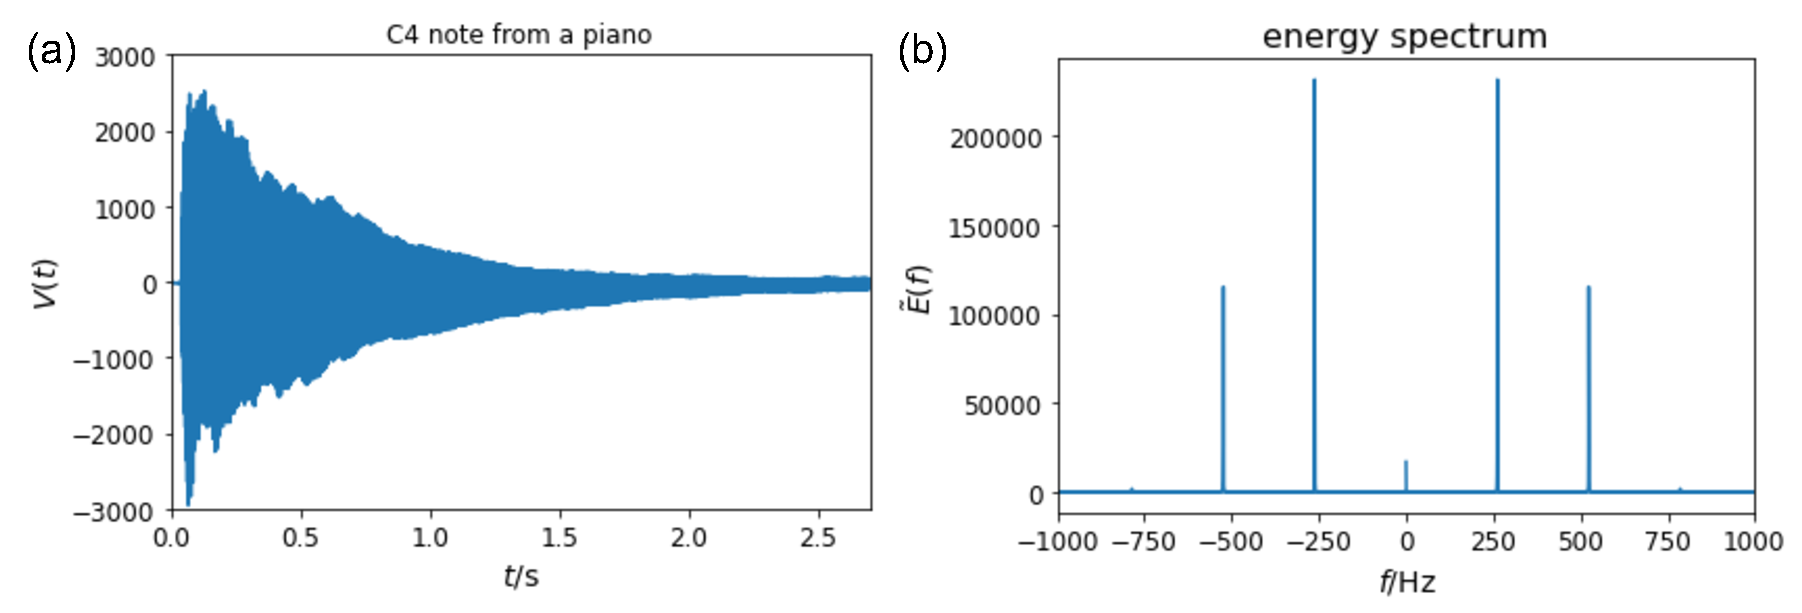
\includegraphics[width=0.9\columnwidth]{./figures/piano-C4.pdf}
\caption{(a) shows a recording of the note C4 from a piano. (Recording duration $\simeq2.7\,\text{s}$.) (b) shows its corresponding energy spectrum.}
\label{fig:piano-C4}
\end{figure}

\section{Analysing sound wave using fast Fourier transform}

TO BE ADDED LATER

\textbf{Question XX.}
Write a code which tells the note of a piano key.

\textbf{Question XX.}
Noise reduction?


\end{document}
